\documentclass[11pt, handout]{beamer}
\usepackage{etex} % Weird problem on dimentions
\usetheme{spensiones}
\usepackage{stata}
\usepackage{tikz, tabularx, ulem}
\usetikzlibrary{arrows, fit,positioning}

\title[{\tt parallel}]{Just tired of endless loops! \\ {\it \footnotesize or} {\normalsize {\tt parallel}: Stata module for parallel computing}}

\author[GGV]{George G. Vega\\ {\tt \scriptsize gvega@spensiones.cl}}
\institute[SPensiones]{Chilean Pension Supervisor}
\def\unix1{Intel Xeon X470 (hexadeca-core)}
\def\windows1{Intel i3 2120 (dual-core)}
\begin{document}

\frame{
\maketitle
{\scriptsize
Thanks to Damian C. Clarke, F\'elix Villatoro and Eduardo Fajnzylber and the Research team of the Chilean Pension Supervisor for their valuable contributions. The usual disclaimers applies.}
}

\frame{
\frametitle{Agenda}
\tableofcontents
}

\section{Motivation}

\begin{frame}[allowframebreaks=.8]
\frametitle{Motivation}
\begin{itemize}[<-+>]
\item Currently home computers are arriving with extremely high computational capabilities. 
\item Motivated by the video games industry, manufacturers have forged a market for low-cost processing units with the number-crunching horsepower comparable to that of a small supercomputer.

\item In the same way, data availability has improved in a significant manner.
\item Big-Data is an active topic by computer scientists and policy-makers
\item Despite of being available (administrative data) to researchers and policy makers, it has not been exploited as it should.
\item The limited use of these social data resources is not a coincidence. issues involving
\begin{itemize}
\item privacy standardized management
\item lack of statistical computing tools
\end{itemize},  and  are still unsolved both for social scientists, and policy-makers. 
\item {\tt parallel} aims to make a contribution to these issues.
\end{itemize}
\end{frame}

\section{Parallel Computing}

\frame{\tableofcontents[currentsection]}

\begin{frame}[allowframebreaks=.8]
\frametitle{Parallel Computing}

\begin{itemize}[<-+>]
\item In simple terms, parallel computing is the simultaneous use of multiple computing resources to solve problems (Barney, 2012)
\item Parallel computing can take place in different levels starting from (a) bit-level, (b) instruction level, (c) data level, up to (d) task level.
\item {\tt parallel} uses data parallelism which basically consists in repeating a task in parallel fashion over independent groups of data.
\item Through parallel computing it is possible to drastically diminish required clock-wall times to complete a computational problem.
\item This is specially important for several scientific areas such as empirical economy, statistics, econometrics and epidemiology.
\end{itemize}

\end{frame}

\section{What is and how does it works}

\frame{\tableofcontents[currentsection]}

\begin{frame}[allowframebreaks=.8]
\frametitle{What is and how does it works}
\framesubtitle{What is?}

\begin{itemize}[<-+>]
\item Inspired in the R library ``snow''.
\item Designed to be used in multicore CPUs (dualcore, quadcore, etc.).
\item {\tt parallel}implements parallel computing methods through an OS's shell scripting (using Stata in batch mode) to accelerate computations.
\item By splitting the dataset into a determined number of clusters this module repeats a task simultaneously over the data-clusters.
\item Depending on the task, {\tt parallel} can reach near to (or over) linear speedups proportional to the number of physical cores the computer has.
\item Thus having a quad-core computer can lead to a 400\% speedup.
\end{itemize}

\end{frame}

\begin{frame}
\frametitle{What is and how does it works}
\framesubtitle{How does it works?}
\begin{figure}
\centering
\scalebox{.65}{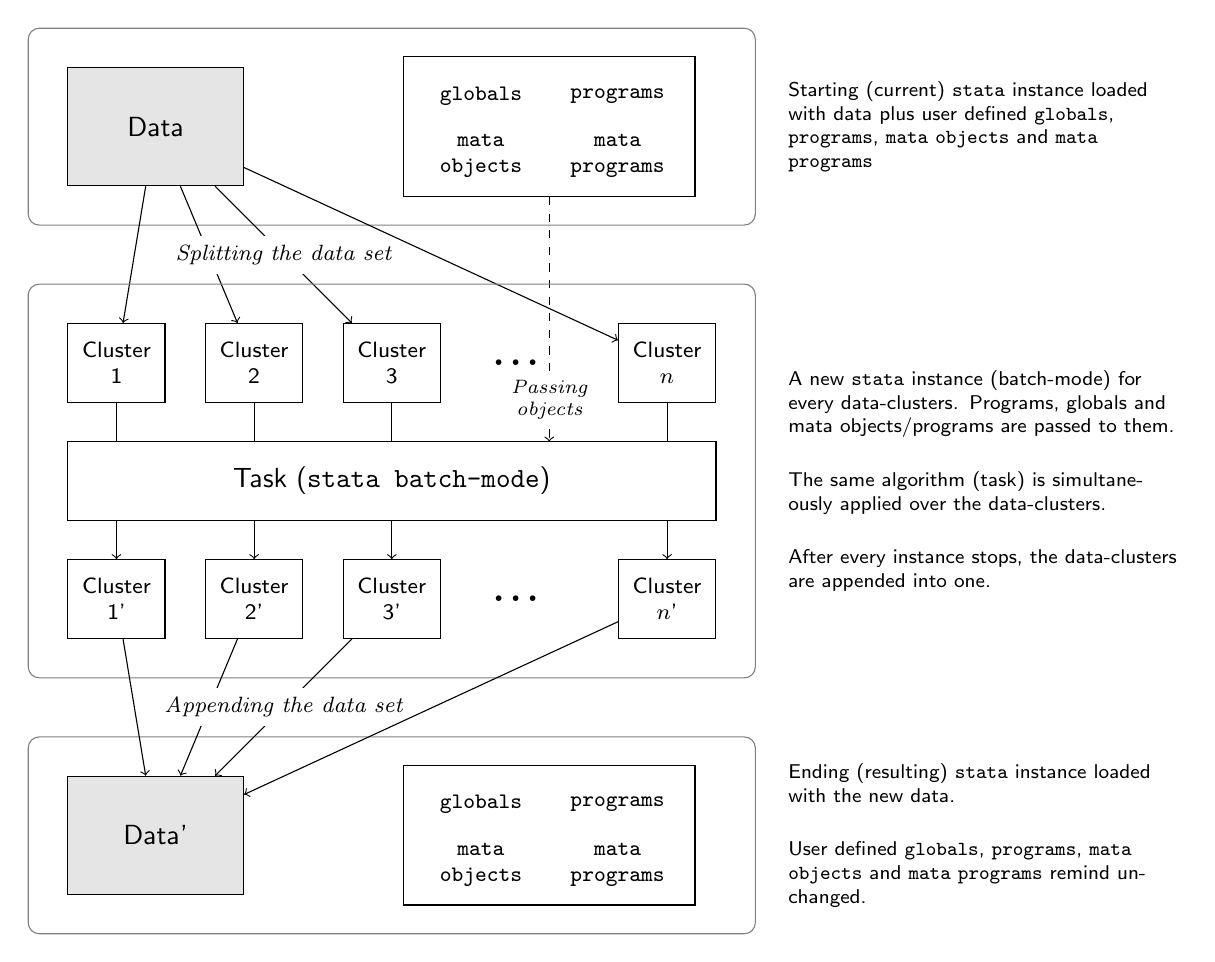
\begin{tikzpicture}[
	every node/.style={node distance=.5cm and .5cm, font=\sffamily}, 
	datablock/.style={rectangle, draw, fill=black!10, text width=2cm, minimum height=1.5cm, text badly centered},
	cluster/.style={rectangle, draw,text width=1cm, text badly centered, minimum height=1cm, font=\footnotesize\sffamily},
	explain/.style={rectangle, text width=5.5cm, align=left, font=\footnotesize\sffamily, node distance=.3, scale=.9}
	] 
	
\node [rectangle, draw=gray, text width=9cm, minimum height=2.5cm, rounded corners] (stata instance0) at (0,0) {};

% Original data
\node [datablock] (data) at (-3,0) {Data};
\matrix [
	draw=black,
	nodes={
		rectangle, text width=1.5cm, minimum height=.75cm, 
		scale=1,
		font=\tt\footnotesize, text badly centered}, column sep=0, row sep=0
	] (others) at (2,0) {
	\node {globals};& \node {programs}; \\
	\node {mata objects}; & \node {mata programs}; \\
};

% Data clusters
\node [cluster] (cluster3) at (0,-3) {Cluster 3};
\node [cluster, left=of cluster3] (cluster2) {Cluster 2};
\node [cluster, left=of cluster2] (cluster1) {Cluster 1};
\node [rectangle, right=of cluster3, text width=1cm, font=\Huge] (threepoints) {...};
\node [cluster, right=of threepoints,text badly centered] (clustern) {Cluster $n$};

% Splitting
\draw[->] (data) -- (cluster1);
\draw[->] (data) -- (cluster2);
\draw[->] (data) -- node [fill=white, font=\footnotesize\it] {Splitting the data set} (cluster3);
\draw[->] (data) -- (clustern);

\draw[->, dashed] (others) -- node [fill=white, font=\scriptsize\it, below=.65cm, text width=1.2cm, minimum height=.7cm,text badly centered] {Passing objects} (2,-4);

% Procesed clusters
\node [cluster] (cluster3p) at (0,-6) {Cluster 3'};
\node [cluster, left=of cluster3p] (cluster2p) {Cluster 2'};
\node [cluster, left=of cluster2p] (cluster1p) {Cluster 1'};
\node [rectangle, right=of cluster3p, text width=1cm, font=\Huge] (threepointsp) {...};
\node [cluster, right=of threepointsp,text badly centered] (clusternp) {Cluster $n$'};

\draw[->] (cluster1) -- (cluster1p);
\draw[->] (cluster2) -- (cluster2p);
\draw[->] (cluster3) -- (cluster3p);
\draw[->] (clustern) -- (clusternp);

% Task
\node [rectangle, draw=gray, text width=9cm, minimum height=5cm, rounded corners] (stata batch) at (0,-4.5) {};
\node [rectangle, fill=white, draw, text width=8cm, text badly centered,minimum height=1cm] (task) at (0,-4.5) {Task (\texttt{stata batch-mode})};

% Result
\node [rectangle, draw=gray, text width=9cm, minimum height=2.5cm, rounded corners] (stata instance1) at (0,-9) {};
\node [datablock] (datap) at (-3,-9) {Data'};
\matrix [
	draw=black,
	nodes={
		rectangle, text width=1.5cm, minimum height=.75cm, 
		scale=1,
		font=\tt\footnotesize, text badly centered}, column sep=0, row sep=0
	] (othersp) at (2,-9) {
	\node {globals};& \node {programs}; \\
	\node {mata objects}; & \node {mata programs}; \\
};

\draw[->] (cluster1p) -- (datap);
\draw[->] (cluster2p) -- (datap);
\draw[->] (cluster3p) -- node [fill=white, font=\footnotesize\it] {Appending the data set} (datap);
\draw[->] (clusternp) -- (datap);

% Text
\node [explain, right=of stata instance0] {Starting (current) {\tt stata} instance loaded with data plus user defined {\tt globals}, {\tt programs}, {\tt mata objects} and {\tt mata programs}};

\node [explain, right=of stata batch] {A new {\tt stata} instance (batch-mode) for every data-clusters. Programs, globals and mata objects/programs are passed to them.\\\bigskip The same algorithm (task) is simultaneously applied over the data-clusters.\\\bigskip After every instance stops, the data-clusters are appended into one.};

\node [explain, right=of stata instance1] {Ending (resulting) {\tt stata} instance loaded with the new data.\\\bigskip User defined {\tt globals}, {\tt programs}, {\tt mata objects} and {\tt mata programs} remind unchanged.};

\end{tikzpicture}}
\end{figure}
\end{frame}

\begin{frame}
\frametitle{What is and how does it works}
{\Large Sounds ``pretty'' but...}\pause {\Huge is this for real!?}
\end{frame}

\section{Benchmarks}
\frame{\tableofcontents[currentsection]}

\begin{frame}
\frametitle{Benchmarks}
\framesubtitle{Simple example}

\begin{table}[!h]
\centering
\caption{Serial replacing using a loop on a Windows Machine (4 clusters)}
\begin{tabular}{l*{3}{c}}\hline
& 100.000 &       1.000.000 &      10.000.000 \\ \hline
CPU &     1.04 &     10.30 &    102.73 \\
Total &     1.39 &      6.97 &     50.85 \\
\hspace{2mm} Setup &     0.00 &      0.00 &      0.00 \\
\hspace{2mm} Compute &     1.33 &      6.76 &     49.11 \\
\hspace{2mm} Finish &     0.06 &      0.21 &      1.74 \\
\hline Ratio (compute) &     0.78 &      1.52 &      2.09 \\
Ratio (total) &     0.75 &      1.48 &      2.02 \\
\hline
\multicolumn{4}{l}{\footnotesize Tested on a \windows1 machine}
\end{tabular}
\end{table}

\end{frame}

\begin{frame}
\frametitle{Benchmarks}
\framesubtitle{Simple example}
\begin{table}[!h]
\centering
\caption{Serial replacing using a loop on a Linux Server (16 clusters)}
\begin{tabular}{l*{3}{c}}\hline
& 100.000 &         1.000.000 &       10.000.000 \\ \hline
CPU &     1.43 &     16.94 &    144.68 \\
Total &     0.34 &      3.20 &     12.49 \\
\hspace{2mm} Setup &     0.00 &      0.00 &      0.00 \\
\hspace{2mm} Compute &     0.32 &      3.07 &     11.54 \\
\hspace{2mm} Finish &     0.02 &      0.12 &      0.95 \\
\hline Ratio (compute) &     4.50 &      5.51 &     12.53 \\
Ratio (total) &     4.22 &      5.30 &     11.58 \\
\hline
\multicolumn{4}{l}{\footnotesize Tested on a \unix1 machine}
\end{tabular}
\end{table}

\end{frame}

\begin{frame}
\frametitle{Benchmarks}
\framesubtitle{Not that simple example}
\begin{table}[!h]
\centering
\caption{Monte Carlo Experiment on a Windows Machine (4 clusters)}
\begin{tabular}{l*{2}{c}}\hline
& 2 &               4 \\ \hline
CPU &   111.49 &    114.13 \\
Total &    58.02 &     37.48 \\
\hspace{2mm} Setup &     0.00 &      0.00 \\
\hspace{2mm} Compute &    58.02 &     37.48 \\
\hspace{2mm} Finish &     0.00 &      0.00 \\
\hline Ratio (compute) &     1.92 &      3.04 \\
Ratio (total) &     1.92 &      3.04 \\
\hline
\multicolumn{3}{l}{\footnotesize Tested on a \windows1 machine}
\end{tabular}
\end{table}
\end{frame}

\begin{frame}
\frametitle{Benchmarks}
\framesubtitle{Not that simple example}

\begin{table}[!h]
\centering
\caption{Monte Carlo Experiment on a Linux Server (16 clusters)}
\begin{tabular}{l*{4}{c}}\hline
& 2 &               4 &               8 &              16 \\ \hline
CPU &   164.79 &    164.04 &    162.84 &    163.89 \\
Total &    69.85 &     34.28 &     19.00 &     10.78 \\
\hspace{2mm} Setup &     0.00 &      0.00 &      0.00 &      0.00 \\
\hspace{2mm} Compute &    69.85 &     34.28 &     19.00 &     10.78 \\
\hspace{2mm} Finish &     0.00 &      0.00 &      0.00 &      0.00 \\
\hline Ratio (compute) &     2.36 &      4.78 &      8.57 &     15.21 \\
Ratio (total) &     2.36 &      4.78 &      8.57 &     15.21 \\
\hline
\multicolumn{4}{l}{\footnotesize Tested on a \unix1 machine}
\end{tabular}
\end{table}

\end{frame}

\begin{frame}
\frametitle{Benchmarks}
\framesubtitle{My favorite... Beats StataMP!}
\begin{table}[!h]
\centering
\caption{Reshaping wide a large database on a Windows Machine (4 clusters)}
\begin{tabular}{l*{3}{c}}\hline
& 100.000 &         1.000.000 &         2.000.000 \\ \hline
CPU &     4.91 &     50.48 &    106.03 \\
Total &     4.42 &     29.00 &     69.69 \\
\hspace{2mm} Setup &     0.45 &      2.06 &      3.51 \\
\hspace{2mm} Compute &     3.84 &     23.57 &     55.86 \\
\hspace{2mm} Finish &     0.13 &      3.37 &     10.31 \\
\hline Ratio (compute) &     1.28 &      2.14 &      1.90 \\
Ratio (total) &     1.11 &      1.74 &      1.52 \\
\hline
\multicolumn{4}{l}{\footnotesize Tested on a \windows1 machine}
\end{tabular}
\end{table}
\end{frame}

\begin{frame}
\frametitle{Benchmarks}
\framesubtitle{My favorite... Beats StataMP!}

\begin{table}[!h]
\centering
\caption{Reshaping wide a large database on a Linux Server (8 clusters)}
\begin{tabular}{l*{3}{c}}\hline
& 100.000 &         1.000.000 &         5.000.000 \\ \hline
CPU &     5.51 &     72.70 &    392.97 \\
Total &     2.33 &     17.46 &     86.44 \\
\hspace{2mm} Setup &     0.00 &      0.00 &      0.00 \\
\hspace{2mm} Compute &     1.83 &     12.42 &     57.93 \\
\hspace{2mm} Finish &     0.50 &      5.04 &     28.51 \\
\hline Ratio (compute) &     3.01 &      5.85 &      6.78 \\
Ratio (total) &     2.37 &      4.16 &      4.55 \\
\hline
\multicolumn{4}{l}{\footnotesize Tested on a \unix1 machine}
\end{tabular}
\end{table}

\end{frame}

\begin{frame}
\frametitle{Benchmarks}
{\Large Ok, it works but...}\pause 

{\Huge it must be really hard to use!}
\end{frame}

\section{Syntax and Usage}

\frame{\tableofcontents[currentsection]}

\begin{frame}
\frametitle{Syntax and Usage}

Setup

\begin{semiverbatim}
\footnotesize
{\bf parallel setclusters} {\it \#}  [, \uline{f}orce] 
\end{semiverbatim}\pause

By syntax

\begin{semiverbatim}
\footnotesize
{\bf parallel} [, by({\it \color{blue} varlist}) \uline{f}orce \uline{k}eep \uline{keepl}ast \uline{p}rograms \uline{m}ata \uline{nog}lobals 

\hspace{1cm} \uline{keept}iming \uline{s}eeds({\it \color{blue} string}) \uline{r}andtype({\it \color{blue} random.org$|$datetime})

\hspace{1cm} \uline{pr}ocessors({\it \color{blue} integer})

\hspace{1cm} \uline{nog}lobal \uline{s}eeds({\it \color{blue} numlist}) \uline{nod}ata]:  {\it stata\_cmd}
\end{semiverbatim}\pause

Do syntax

\begin{semiverbatim}
\footnotesize
{\bf parallel do} {\it \color{blue} filename}

\hspace{1cm} [, by({\it \color{blue} varlist}) \uline{f}orce \uline{k}eep \uline{keepl}ast \uline{p}rograms \uline{m}ata \uline{nog}lobals 

\hspace{1cm} \uline{keept}iming \uline{s}eeds({\it \color{blue} string}) \uline{r}andtype({\it \color{blue} random.org$|$datetime})

\hspace{1cm} \uline{pr}ocessors({\it \color{blue} integer})

\hspace{1cm} \uline{nog}lobal \uline{s}eeds({\it \color{blue} numlist}) \uline{nod}ata] 
\end{semiverbatim}

\end{frame}


\begin{frame}
\frametitle{Syntax and Usage}\framesubtitle{setup}
\begin{stlog}
. sysuse bplong.dta
(fictional blood-pressure data)
{\smallskip}
. sort patient
{\smallskip}
. parallel setclusters 4
N Clusters: 4
Stata dir:  /usr/local/stata12/stata-se
{\smallskip}

\end{stlog}

\end{frame}

\begin{frame}
\frametitle{Syntax and Usage}\framesubtitle{egen by}
\footnotesize
\begin{stlog}
. bysort patient: egen max_bp = max(bp)
{\smallskip}
. parallel, by(patient) nog: by patient: egen max_bp_pll = max(bp)
Parallel Computing with Stata (by GVY)
Clusters: 4
ID: 9lhcit1mkx
{\smallskip}
[1] 31269
Stata instances PID:
[1] 31279
[2] 31280
[3] 31281
[4] 31282
{\sltt{cluster 1}} has finished without any error...
{\sltt{cluster 2}} has finished without any error...
{\sltt{cluster 3}} has finished without any error...
{\sltt{cluster 4}} has finished without any error...
{\smallskip}
. summ max_bp*
{\smallskip}
    Variable {\VBAR}       Obs        Mean    Std. Dev.       Min        Max
\HLI{13}{\PLUS}\HLI{56}
      max_bp {\VBAR}       240    160.8333    11.56993        138        185
  max_bp_pll {\VBAR}       240    160.8333    11.56993        138        185
{\smallskip}

\end{stlog}

\end{frame}

\begin{frame}[allowframebreaks=1]
\frametitle{Syntax and Usage}\framesubtitle{reshape}
\begin{stlog}
. qui reshape wide bp max_bp*, i(patient) j(when)
{\smallskip}
. summ 
{\smallskip}
    Variable {\VBAR}       Obs        Mean    Std. Dev.       Min        Max
\HLI{13}{\PLUS}\HLI{56}
     patient {\VBAR}       120        60.5    34.78505          1        120
         bp1 {\VBAR}       120      156.45    11.38985        138        185
     max_bp1 {\VBAR}       120    160.8333    11.59421        138        185
 max_bp_pll1 {\VBAR}       120    160.8333    11.59421        138        185
         bp2 {\VBAR}       120    151.3583    14.17762        125        185
\HLI{13}{\PLUS}\HLI{56}
     max_bp2 {\VBAR}       120    160.8333    11.59421        138        185
 max_bp_pll2 {\VBAR}       120    160.8333    11.59421        138        185
         sex {\VBAR}       120          .5    .5020964          0          1
      agegrp {\VBAR}       120           2    .8199201          1          3
{\smallskip}
. qui reshape long
{\smallskip}
. qui parallel, by(patient) f nog: reshape wide bp max_bp*, i(patient) j(when)
{\smallskip}
. return list
{\smallskip}
scalars:
              r(pll_n) =  4
         r(pll_t_fini) =  .003
         r(pll_t_calc) =  .323
         r(pll_t_setu) =  0
         r(pll_t_reps) =  1
           r(pll_errs) =  0
{\smallskip}
macros:
             r(pll_id) : "r1c9jesifd"
            r(pll_dir) : "/u1/users/estudios/investigacion/george/comandos_paqu
> etes_librerias/stata/parallel"
{\smallskip}
. summ
{\smallskip}
    Variable {\VBAR}       Obs        Mean    Std. Dev.       Min        Max
\HLI{13}{\PLUS}\HLI{56}
     patient {\VBAR}       120        60.5    34.78505          1        120
         bp1 {\VBAR}       120      156.45    11.38985        138        185
     max_bp1 {\VBAR}       120    160.8333    11.59421        138        185
 max_bp_pll1 {\VBAR}       120    160.8333    11.59421        138        185
         bp2 {\VBAR}       120    151.3583    14.17762        125        185
\HLI{13}{\PLUS}\HLI{56}
     max_bp2 {\VBAR}       120    160.8333    11.59421        138        185
 max_bp_pll2 {\VBAR}       120    160.8333    11.59421        138        185
         sex {\VBAR}       120          .5    .5020964          0          1
      agegrp {\VBAR}       120           2    .8199201          1          3
{\smallskip}

\end{stlog}

\end{frame}

\begin{frame}
\frametitle{Syntax and Usage}\framesubtitle{{\tt parallel do} syntax}

Imagine that we have a model that requires looping over each and every record of a panel-data dataset.\pause

\begin{semiverbatim}

\hspace{1cm}. use mybigpanel.dta, clear

\hspace{1cm}. parallel setclusters 4

\hspace{1cm}. parallel do mymodel.do, by(timevar panelvar)
    
\hspace{1cm}. collapse ...
\end{semiverbatim}   \pause

where {\tt mymodel.do} would look something like this \pause

\begin{semiverbatim}
\hspace{1cm}local maxiter = \_N

\hspace{1cm}forval i = 1/`maxiter' \{

\hspace{2cm}...some routine...

\hspace{1cm}\}
\end{semiverbatim}
\end{frame}

\section{Concluding Remarks}

\begin{frame}
\frametitle{Concluding Remarks}

\begin{itemize}[<-+>]
\item In the case of Stata, {\tt parallel} is, to the authors knowledge, the first public user-contribution to parallel computing
\item The major benefits, measured in terms of speedups, can be reached by simulation models and non-vectorized operations such as control-flow statements.
\item Speed gains are directly related to the proportion of the algorithm that can be de-serialized and the number of processors with which the parallelization is made, making possible reach near to constant scale improvements.
\item The simplicity of this type of parallelism, giving to its easy way, it seems like a worthy activity for a wide range of social scientists and researchers.
\end{itemize}

\end{frame}

\frame{\maketitle}

\end{document}